\documentclass[a4paper]{article}

\usepackage[T1]{fontenc}
\usepackage{titling}
\usepackage[polish]{babel}
\usepackage{multirow}
\selectlanguage{polish}
\usepackage[utf8]{inputenc}
\usepackage{amsmath}
\usepackage{listings}
\usepackage{graphicx}
\usepackage{framed}
\usepackage{fullpage}
\usepackage{adjustbox}


\setlength{\droptitle}{+10em}
\title{\huge
  Obliczenia naukowe \\
  \large Lista 2}
\author{Arkadiusz Ziobrowski \\ 229728}
\date{}

\begin{document}
\maketitle

\pagebreak




\section{Zadanie pierwsze}

\subsection{Opis problemu}
\paragraph{}
Celem zadania była modyfikacja danych wejściowych zadania 5 z listy 1 i zaobserwowanie jaki wpływ na wyniki działania algorytmów liczenia iloczynu skalarnego mają takie zmiany.
\subsection{Rozwiązanie}
\paragraph{}
Do wykonania zadania zostały użyte zaimplementowane w zadaniu 5 z listy 1 algorytmy liczenia iloczynu skalarnego. Jedynymi wprowadzonymi zmianami były modyfikacje danych wejściowych. W wektorze $x$ wartość $x_{4} = 0.5772156649$ została zmieniona na $x'_{4} = 0.577215664$, zaś z $x_{5} = 0.3010299957$ została usunięta ostatnia $7$, co dało wartość $x'_{5} = 0.301029995$. 

\subsection{Wyniki i interpretacja}
\paragraph{}
\begin{center}
 \begin{tabular}{ |c | c | c | c | c|  }
 \hline
 \multicolumn{5}{|c|}{Wyniki algorytmów} \\
 \hline
 \multirow{2}{*}{Nazwa algorytmu} & \multicolumn{2}{|c|}{Dane oryginalne} & \multicolumn{2}{|c|}{Dane zmodyfikowane} \\
  \cline{2-5}
 &\texttt{Float32} & \texttt{Float64} & \texttt{Float32} & \texttt{Float64}\\
 \hline
 Algorytm 1 & -0.4999443 & 1.0251881368296672e-10 & -0.4999443 & -0.004296342739891585\\
 Algorytm 2 & -0.4543457 & -1.5643308870494366e-10 & -0.4543457 & -0.004296342998713953\\
 Algorytm 3 & -0.5 & 0.0 & -0.5 & -0.004296342842280865\\
 Algorytm 4 & -0.5 & 0.0 & -0.5 & -0.004296342842280865\\
 \hline
\end{tabular}
\end{center}

W powyższej tabeli można zauważyć, iż mimo zmiany danych wejściowych, wyniki działania algorytmów liczenia iloczynu skalarnego nie zmieniły się dla arytmetyki \texttt{single}. Przyjrzyjmy się reprezentacji bitowej wartości $x'_{4}$ oraz $x'_{5}$.

\begin{center}
\begin{tabular}{ |c|c| } 
 \hline
 $x_{4}$ & 0 01111110 00100111100010001101000 \\ 
 $x'_{4}$ & 0 01111110 00100111100010001101000 \\ 
 $x_{5}$ & 0 01111101 00110100010000010011011 \\
 $x'_{5}$ & 0 01111101 0011010001000001001101\textbf{0} \\ 
 \hline
\end{tabular}
\end{center}

Identyczne wyniki działania algorytmów w arytmetyce \texttt{single} wynikają z precyzji tej arytmetyki. Reprezentacja bitowa wartości $x_{4}$ jest taka sama jak $x'_{4}$, a $x_{5}$ różni się od $x'_{5}$ na najmniej znaczącym bicie. Powoduje to, że obliczenia w arytmetyce \texttt{Float32} odbywają się na niemal identycznych wartościach, stąd też wystąpienie niezmienionych wyników, mimo modyfikacji danych wejściowych.

Natomiast dla arytmetyki \texttt{double} różnice w wynikach są doskonale widoczne. Dla Algorytmu 3 oraz Algorytmu 4 nie pojawiają się już wartości zerowe. Otrzymane wyniki różnią się jednak wciąż w dużym stopniu od wyników oczekiwanych. Można zaobserwować również pewną stabilizację wyników po zmianie danych wejściowych. Wyniki działania algorytmów są podobne, w przeciwieństwie do wyników odpowiadających danym oryginalnym. Dla powyższych danych jedynie zmiana $x'_{4}$ na $x_{4}$ oraz $x'_{5}$ na $x_{5}$ spowodowała duże odchylenia wyników od ustabilizowanych wartości. 
\subsection{Wnioski}
\paragraph{}
Małe zmiany danych wejściowych dla arytmetyki \texttt{single} nie zawsze muszą powodować zmiany w wynikach obliczeń. Spowodowane jest to precyzją tej arytmetyki. W przypadku arytmetyki \texttt{double} widoczne jest, że małe zmiany danych wejściowych podczas obliczeń na wektorach niemal prostopadłych powodują znaczne odchylenia wyników. Obliczanie iloczynu skalarnego dla $x = (x_{1}, ..., x_{n})$, $y = (y_{1}, ..., y_{n})$, gdzie 
niektóre $sgn(x_{i}) \neq sgn(y_{i})$ jest zatem źle uwarunkowane, gdyż małe zmiany danych powodują duże odkształcenia wyników.
\pagebreak

\section{Zadanie drugie}

\subsection{Opis problemu}
\paragraph{}
Celem zadania było narysowanie wykresów funkcji $f(x) = e^xln(1 + e^{-x})$ w co najmniej dwóch programach do wizualizacji. Następnie należało porównać otrzymane wykresy z wyliczoną granicą funkcji $\lim_{x \to \infty} f(x)$.

\subsection{Rozwiązanie}
\paragraph{}
Wykresy wygenerowane zostały przy użyciu narzędzi do wizualizacji \textit{gnuplot} oraz \textit{Gadfly}.
W celu wygenerowania wykresu funkcji w programie \textit{gnuplot} została wykonana następująca komenda:
\begin{center}
\texttt{gnuplot> plot [-15 : 45] exp(x)*log(1 + exp(-x))}
\end{center}

W celu wygenerowania wykresu funkcji przy użyciu narzędzia \textit{Gadfly} został napisany program w języku \texttt{Julia}.
\begin{center}
\begin{lstlisting}[frame = single]
using Gadfly
f(x) = e^x * log(1 + e^-x)
draw(PDF("gadfly.pdf", 654mm, 350mm), plot(f, -15, 45))
\end{lstlisting}
\end{center}

\subsection{Wyniki i interpretacja}
\paragraph{}
\begin{figure}[htbp]
  \centering
  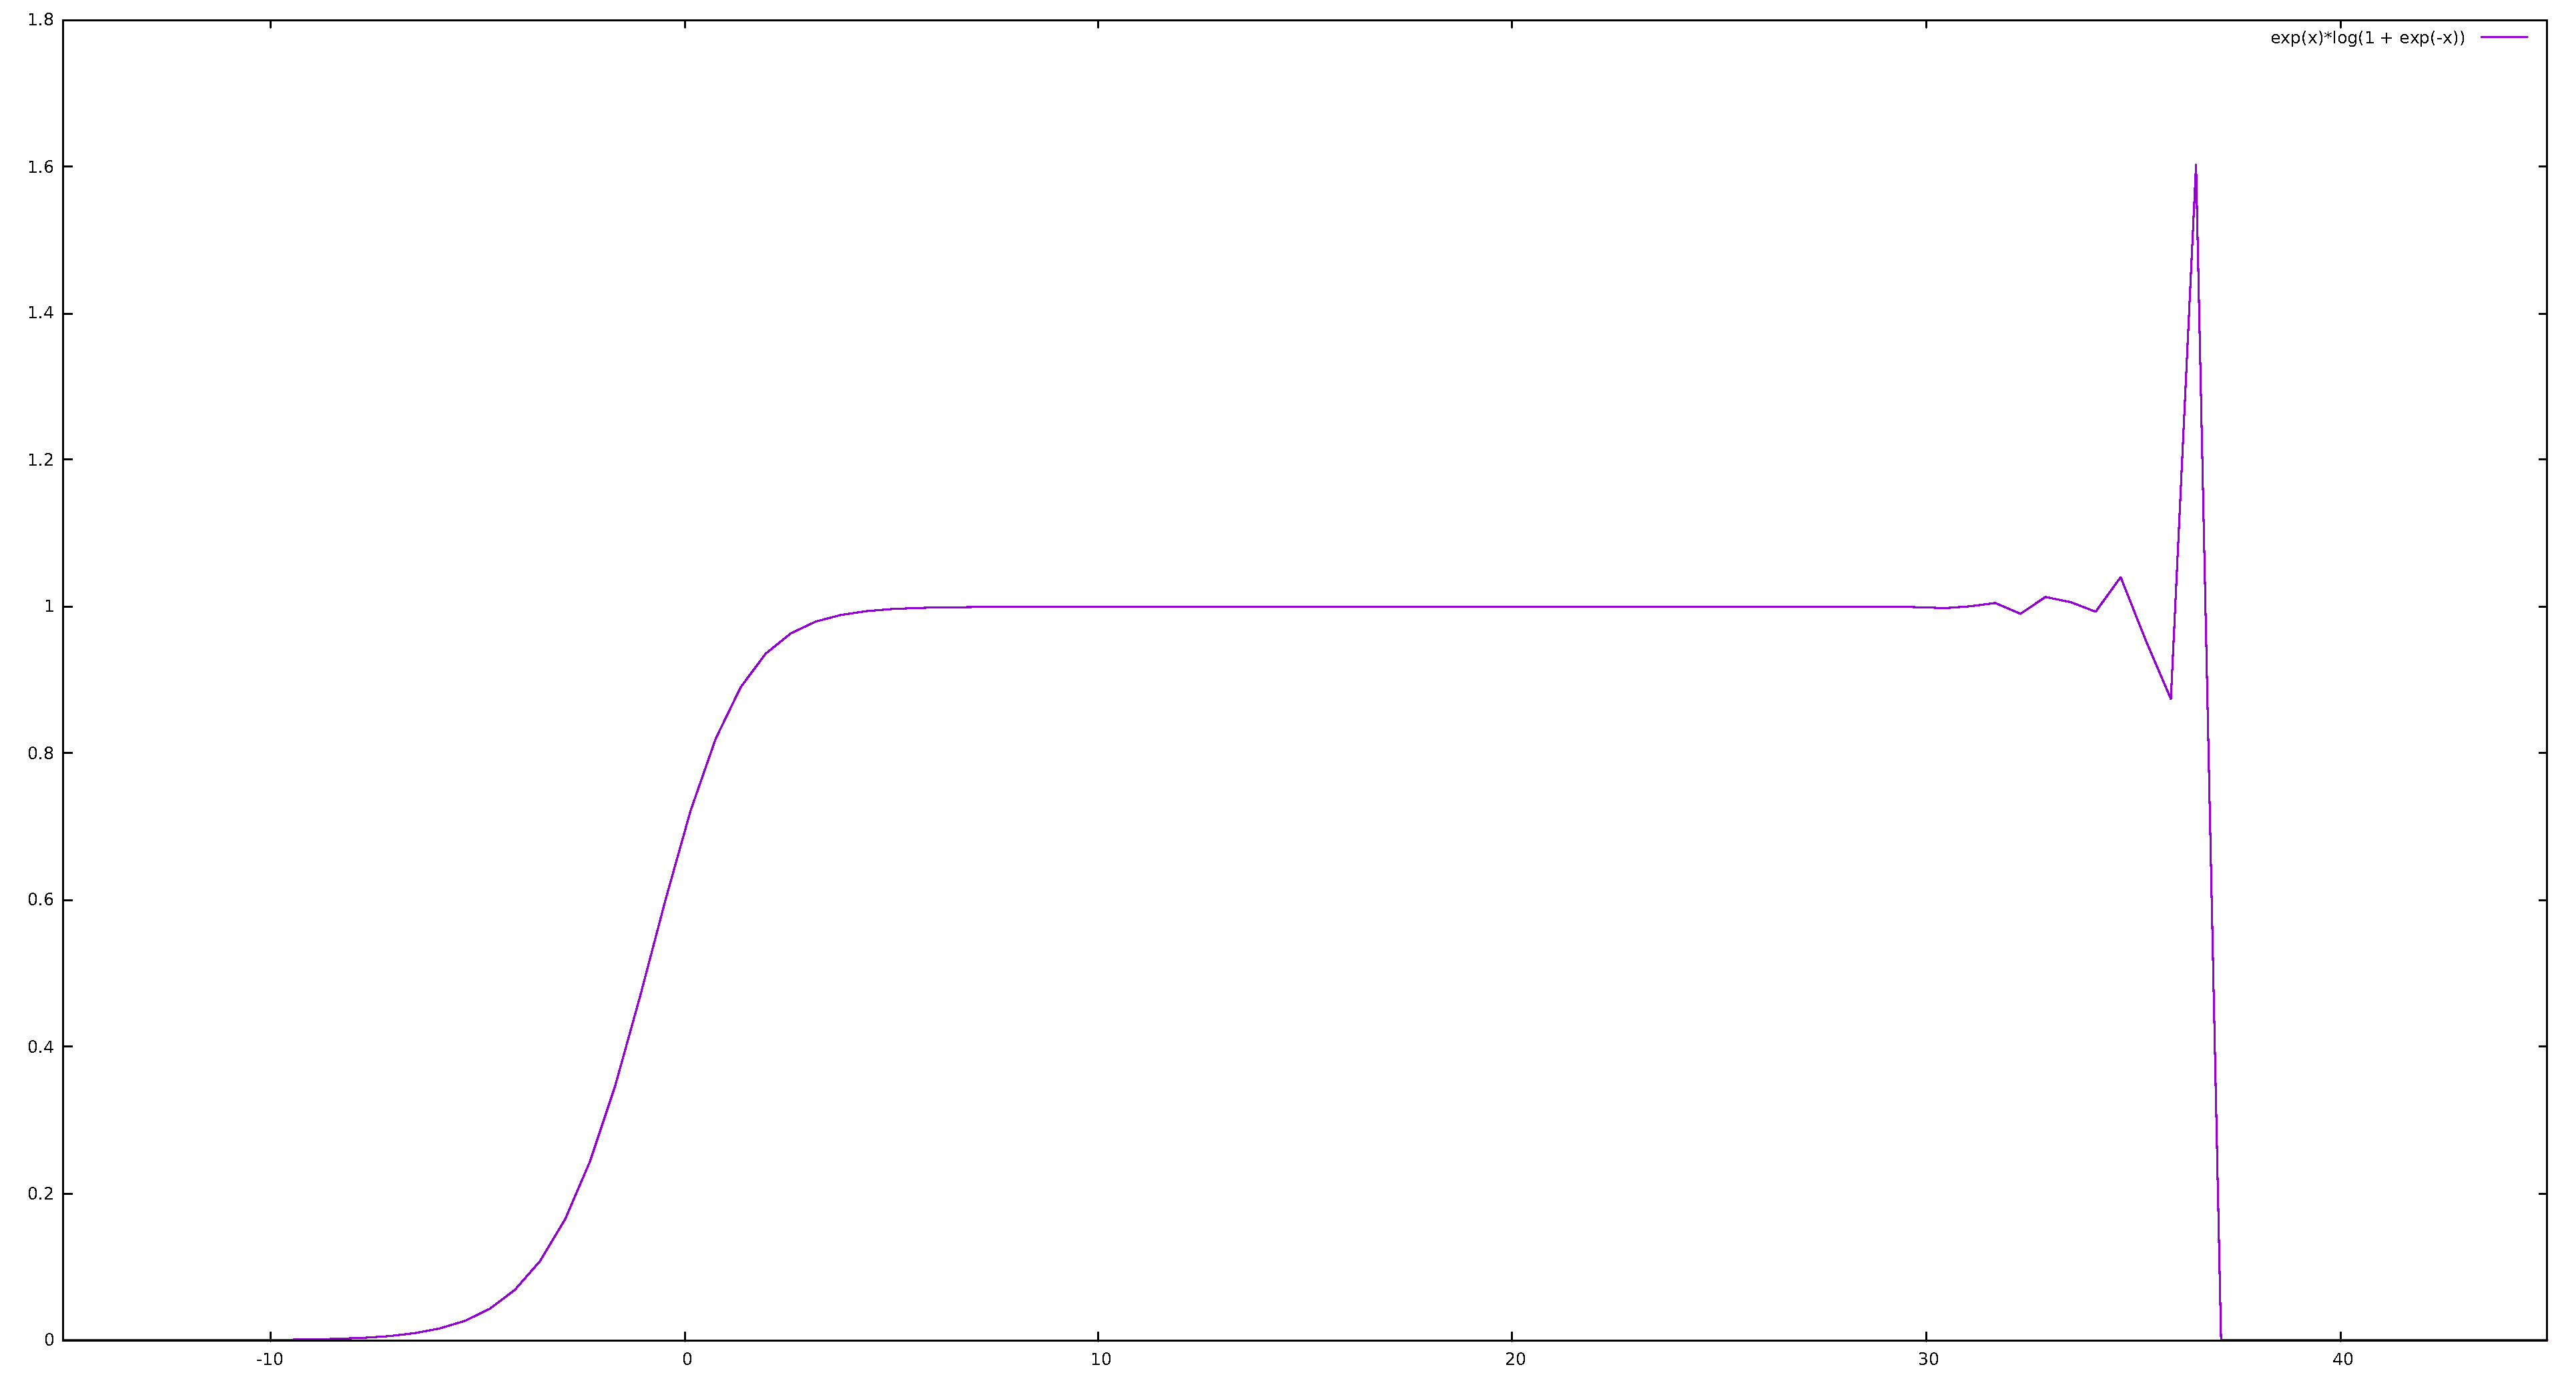
\includegraphics[scale=0.25]{gnuplot.pdf}
  \caption{$f(x) = e^xln(1 + e^{-x})$ w \textit{gnuplot}}
\end{figure}
\clearpage
\begin{figure}[htbp]
  \centering
  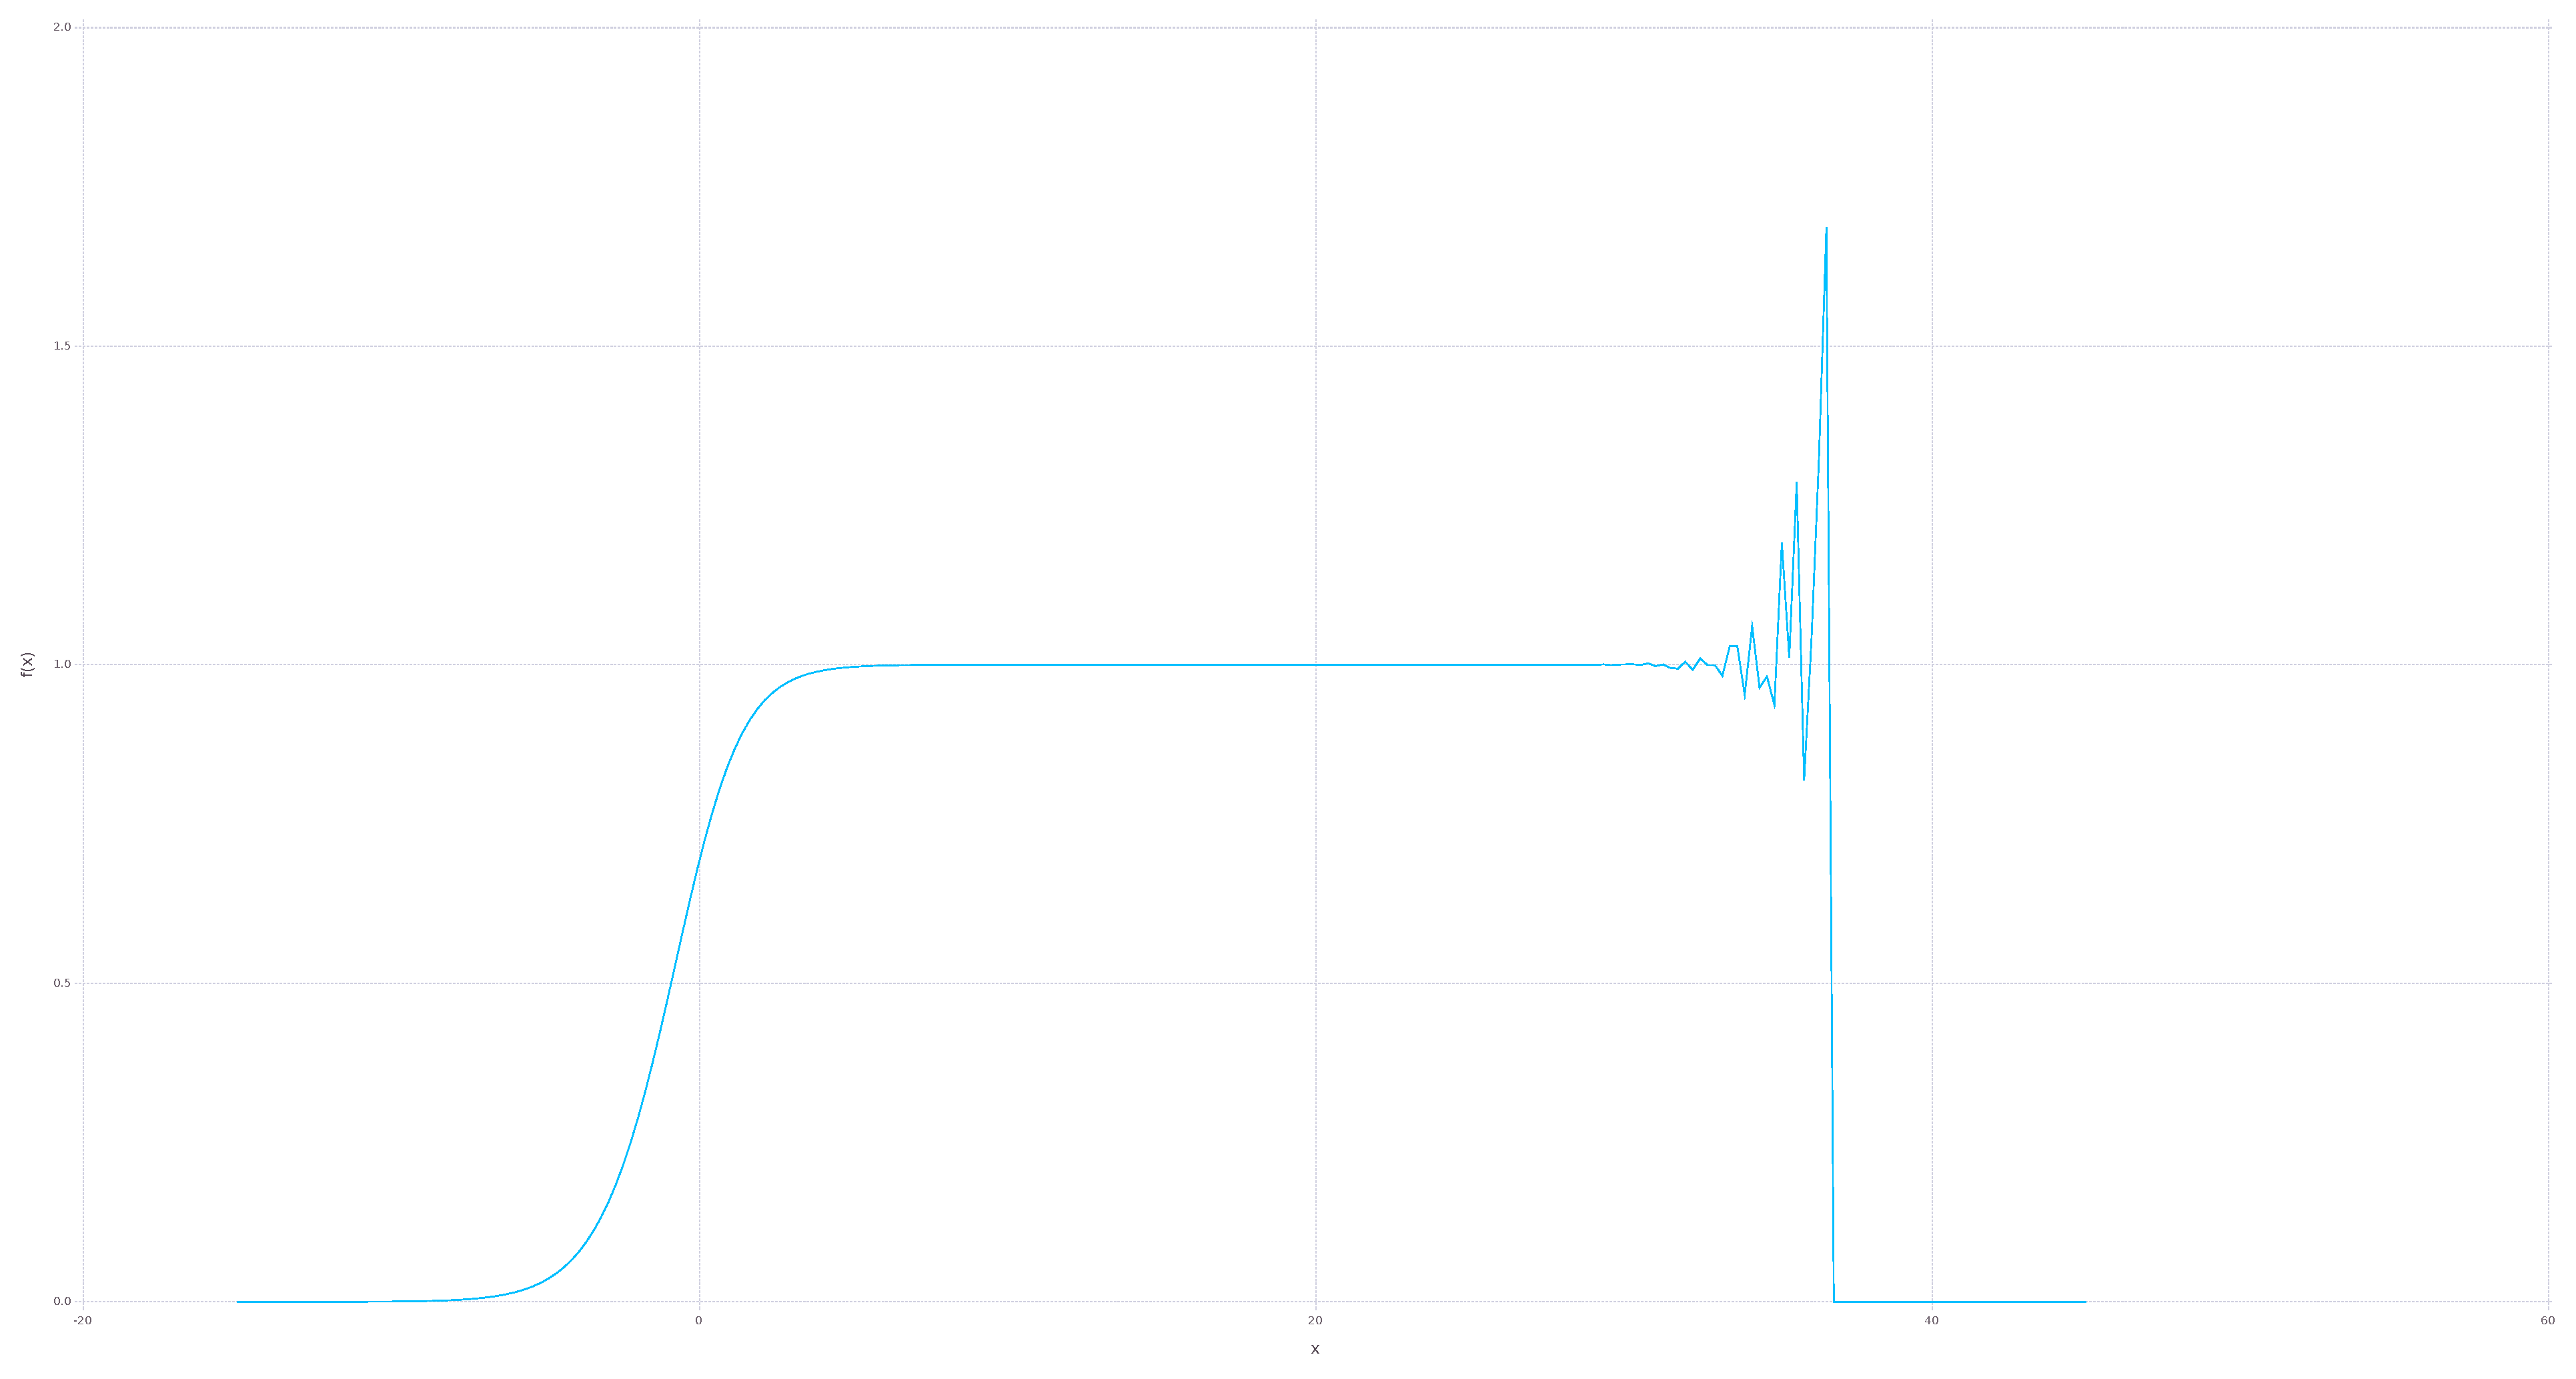
\includegraphics[scale=0.25]{gadfly.pdf}
  \caption{$f(x) = e^xln(1 + e^{-x})$ w \textit{Gadfly}}
\end{figure}

Wyliczona granica $\lim_{x \to \infty} f(x) = 1$. Na wykresach widoczne jest, że zachowanie funkcji różni się od wartości granicy. Zbieżność funkcji na wykresie do 0 jest spowodowane przez $ln(1 + e^{-x})$. Dla dużych $x$ wartość $1 + e^{-x} = 1$, natomiast $ln(1) = 0$. Stąd dla dużych $x$ $f(x) = e^xln(1) = e^x * 0 = 0$. Również widoczne przed gwałtownym spadkiem do $0$ zaburzenie jest spowodowane redukcją cyfr znaczących dla $1 + e^{-x}$.
\subsection{Wnioski}
\paragraph{}
Wykresy niektórych funkcji nie mogą być przedstawione dokładnie na całym przedziale z powodu występowania zjawiska redukcji cyfr znaczących. Stąd też różnica między wartością granicy funkcji, a rzeczywistym jej zachowaniem w reprezentacji w artymetyce \texttt{double}. Należy być wyczulonym na występowanie tego zjawiska, gdyż poprawne z matematycznego punktu widzenia założenia, nie zawsze znajdują pokrycie w realizacji komputerowej.
\section{Zadanie trzecie}

\subsection{Opis problemu}
\paragraph{}
Celem zadania było rozwiązanie układu równań liniowych $\textbf{Ax = b}$ dla $\textbf{A}$ będącego macierzą Hilberta stopnia $n$ oraz macierzą losową stopnia $n$ o zadanym wskaźniku uwarunkowania. Układy miały być rozwiązane za pomocą dwóch algorytów: eliminacji Gaussa oraz $x = A^{-1}b$.

\subsection{Rozwiązanie}
\paragraph{}
Rozwiązywanie układu równań liniowych zaczynamy od wygenerowania macierzy Hilberta, bądź macierzy losowej przy użyciu odpowiednio funkcji \texttt{hilb(n)} i \texttt{matcond(n, c)}, gdzie \texttt{n} to stopień macierzy, a \texttt{c} zadany wskaźnik uwarunkowania. Następnie tworzymy $x = (1, ..., 1)^T$ i $b = (0, ..., 0)^T$ przy użyciu funkcji \texttt{ones(n)} oraz \texttt{zeros(n)} z języka \texttt{Julia}. Wektor prawych stron otrzymujemy poprzez wykonanie \texttt{b = A * x}. Teraz przystępujemy do rozwiązywania układu równań liniowych. Macierze, na których operujemy muszą być nieosobliwe. Macierz Hilberta jest nieosobliwa, ale w przypadku macierzy losowej dodatkowo sprawdzamy czy $det(A) \neq 0$. Układy równań rozwiązujemy poprzez zastosowanie eliminacji Gaussa (w języku \texttt{Julia} używamy \texttt{x = A\textbackslash b}, ponieważ operator \texttt{\textbackslash} jest dociążony) oraz $x = A^{-1}b$.
\subsection{Wyniki i interpretacja}
\paragraph{}

Przez $\delta$ oznaczony jest błąd względny liczony jako $ \frac{||x - x'||}{||x||}$.
\begin{center}
 \begin{tabular}{ |c | c | c | c | c|  }
 \hline
 \multicolumn{5}{|c|}{Macierz Hilberta} \\
 \hline
 n & rank(A) & cond(A) & $\delta (A\textbackslash b)$ & $\delta (A^{-1}b)$ \\
 \hline
 1 & 1 & 1.0 & 0.0 & 0.0 \\
2 & 2 & 19.28147006790397 & 5.661048867003676e-16 & 1.4043333874306803e-15 \\
3 & 3 & 524.0567775860644 & 8.022593772267726e-15 & 0.0 \\
4 & 4 & 15513.73873892924 & 4.137409622430382e-14 & 0.0 \\
5 & 5 & 476607.25024259434 & 1.6828426299227195e-12 & 3.3544360584359632e-12 \\
6 & 6 & 1.4951058642254665e7 & 2.618913302311624e-10 & 2.0163759404347654e-10 \\
7 & 7 & 4.75367356583129e8 & 1.2606867224171548e-8 & 4.713280397232037e-9 \\
8 & 8 & 1.5257575538060041e10 & 6.124089555723088e-8 & 3.07748390309622e-7 \\
9 & 9 & 4.931537564468762e11 & 3.8751634185032475e-6 & 4.541268303176643e-6 \\
10 & 10 & 1.6024416992541715e13 & 8.67039023709691e-5 & 0.0002501493411824886 \\
11 & 11 & 5.222677939280335e14 & 0.00015827808158590435 & 0.007618304284315809 \\
12 & 11 & 1.7514731907091464e16 & 0.13396208372085344 & 0.258994120804705 \\
13 & 11 & 3.344143497338461e18 & 0.11039701117868264 & 5.331275639426837 \\
14 & 12 & 6.200786263161444e17 & 1.4554087127659643 & 8.71499275104814 \\
15 & 12 & 3.674392953467974e17 & 4.696668350857427 & 7.344641453111494 \\
16 & 12 & 7.865467778431645e17 & 54.15518954564602 & 29.84884207073541 \\
17 & 12 & 1.263684342666052e18 & 13.707236683836307 & 10.516942378369349 \\
18 & 12 & 2.2446309929189128e18 & 9.134134521198485 & 7.575475905055309 \\
19 & 13 & 6.471953976541591e18 & 9.720589712655698 & 12.233761393757726 \\
20 & 13 & 1.3553657908688225e18 & 7.549915039472976 & 22.062697257870493 \\
 \hline
\end{tabular}
\end{center}
Macierz Hilberta jest przykładem macierzy bardzo źle uwarunkowanej. Wskaźnik uwarunkowania dla macierzy Hilberta $H_{n}$ wynosi dla $cond(H_{6}) = 1.5e7$, a dla $cond(H_{10}) = 1.5e13$. Im większy wskaźnik uwarunkowania tym wyniki stają się mniej wiarygodne. Jak widać w powyższej tabeli, wskaźnik uwarunkowania dla macierzy Hilberta rośnie bardzo szybko, przez co nawet dla niewielkich $n$ rozwiązania stają się niepoprawne. Liczone błędy względne rosną bardzo szybko dla wyników działania obu algorytmów.
\begin{center}
 \begin{tabular}{ |c | c | c | c | c|  }
 \hline
 \multicolumn{5}{|c|}{Macierz losowa o zadanym wskaźniku uwarunkowania} \\
 \hline
 n & rank(A) & cond(A) & $\delta (A\textbackslash b)$ & $\delta (A^{-1}b)$ \\
 \hline
 5 & 5 & 1.0 & 1.719950113979703e-16 & 1.4043333874306804e-16 \\
5 & 5 & 10.0 & 2.6272671962866383e-16 & 1.719950113979703e-16 \\
5 & 5 & 1000.0 & 1.0295066439664222e-14 & 1.0173423748423966e-14 \\
5 & 5 & 1.0e7 & 4.330021001082515e-11 & 1.0732962350934844e-10 \\
5 & 5 & 1.0e12 & 2.522301895949992e-6 & 4.264961199760036e-6 \\
5 & 4 & 1.0e16 & 0.004509893783428691 & 0.06702378309227254 \\
10 & 10 & 1.0 & 3.2368285245694683e-16 & 3.528343968566428e-16 \\
10 & 10 & 10.0 & 2.673771110915334e-16 & 1.7901808365247238e-16 \\
10 & 10 & 1000.0 & 1.0870438501801568e-14 & 7.303883810382728e-15 \\
10 & 10 & 1.0e7 & 1.6290627639144684e-10 & 2.1344738145604099e-10 \\
10 & 10 & 1.0e12 & 6.221212756561689e-16 & 7.635352669238318e-6 \\
10 & 9 & 1.0e16 & 4.496060575246782e-16 & 0.07733980419227864 \\
20 & 20 & 1.0 & 7.842607901964165e-16 & 4.896322696446008e-16 \\
20 & 20 & 10.0 & 2.8413902102441497e-16 & 5.283775210381055e-16 \\
20 & 20 & 1000.0 & 1.0986468849098833e-14 & 9.99348740935716e-15 \\
20 & 20 & 1.0e7 & 2.4285867112639743e-10 & 2.557721613880287e-10 \\
20 & 20 & 1.0e12 & 2.9043168599769948e-5 & 2.724071818393436e-5 \\
20 & 19 & 1.0e16 & 0.2069677081502989 & 0.26486564253173717 \\
 \hline
\end{tabular}
\end{center}
Macierz losowa o zadanym wskaźniku uwarunkowania potwierdza obserwacje zależności między wskaźnikiem uwarunkowania a $\delta$ z macierzy Hilberta. Można tutaj dokładnie obejrzeć wpływ wzrastającego, kontrolowanego wskaźnika uwarunkowania na generowane błędy względne. Wraz ze zwiększeniem $cond(A)$ rosną błędy względne algorytmów rozwiązywania układu równań liniowych dla macierzy o zadanym $n$.
\subsection{Wnioski}
\paragraph{}
Macierze o wysokim wskaźniku uwarunkowania generują duże błędy w obliczeniach. Pojawienie się macierzy Hilberta podczas obliczeń może sprawić, że otrzymane wyniki będą niewiarygodne. Na szczególną uwagę zasługuje stopień „złośliwości” macierzy Hilberta. Dla macierzy $H_{20}$ wskaźnik uwarunkowania wynosi aż $1.3553657908688225e18$.
\section{Zadanie czwarte}

\subsection{Opis problemu}
\paragraph{}
Celem zadania było sprawdzenie zachowania pierwiastków wielomianu Wilkinsona dla wielomianów postaci naturalnej:

\begin{center}
$P(x) = x^{20} - 210x^{19} + 20615x^{18} - 1256850x^{17} + 53327946x^{16} - 1672280820x^{15} + 40171771630x^{14} - 756111184500x^{13} + 11310276995381x^{12} - 135585182899530x^{11} + 1307535010540395x^{10} - 10142299865511450x^9 + 63030812099294896x^8 - 311333643161390640x^7 + 1206647803780373360x^6 - 3599979517947607200x^5 + 8037811822645051776x^4 - 12870931245150988800x^3 + 13803759753640704000x^2 - 8752948036761600000x + 2432902008176640000$
\end{center}
oraz postaci iloczynowej:
\begin{center}
$p(x) = (x - 20)(x - 19)(x - 18)(x - 17)(x - 16)(x - 15)(x - 14)(x - 13)(x - 12)(x - 11)(x - 10)(x - 9)(x - 8)(x - 7)(x - 6)(x - 5)(x - 4)(x - 3)(x - 2)(x - 1)$
\end{center}

Drugą częścią zadania było wprowadzenie zaburzenia dla wielomianu w postaci naturalnej dla współczynnika przy $x^{19}$ i sprawdzenie zmiany zachowania pierwiastków wielomianu.
\subsection{Rozwiązanie}
\paragraph{}
Badanie zachowania pierwiastków wielomianu Wilkinsona zaczynamy od stworzenia postaci naturalnej wielomianu w języku \texttt{Julia}. Współczynniki wielomianu przechowujemy w tablicy. Wielomian Wilkinsona w postaci naturalnej tworzymy poprzez użycie konstruktora \texttt{Poly} z pakietu \texttt{Polynomials}. Postać iloczynową tworzymy przy użyciu funkcji \texttt{poly}. Ważne jest, aby przekazywane do metod \texttt{poly} oraz \texttt{Poly} współczynniki były uporządkowane od współczynników stojących przy najniższych potęgach $x$. Pierwiastki wielomianu wyliczamy przy użyciu funkcji \texttt{roots}, a wartość wielomianu dla danego argumentu $x$ za pomocą metody \texttt{polyval}.
\clearpage
\subsection{Wyniki i interpretacja}
\paragraph{}

W poniższej tabeli przez $z_{k}$ zostały oznaczone wyliczone pierwiastki wielomianu, a przez $k$ dokładne pierwiastki.
\begin{center}
 \begin{tabular}{ |c | c | c | c|  }
 \hline
 $z_{k}$ & $|P(z_{k})|$ & $|p(z_{k})|$ & $|z_{k} - k|$ \\
 \hline
 0.9999999999996989 & 36352.0 & 38400.0 & 3.0109248427834245e-13 \\
2.0000000000283182 & 181760.0 & 198144.0 & 2.8318236644508943e-11 \\
2.9999999995920965 & 209408.0 & 301568.0 & 4.0790348876384996e-10 \\
3.9999999837375317 & 3.106816e6 & 2.844672e6 & 1.626246826091915e-8 \\
5.000000665769791 & 2.4114688e7 & 2.3346688e7 & 6.657697912970661e-7 \\
5.999989245824773 & 1.20152064e8 & 1.1882496e8 & 1.0754175226779239e-5 \\
7.000102002793008 & 4.80398336e8 & 4.78290944e8 & 0.00010200279300764947 \\
7.999355829607762 & 1.682691072e9 & 1.67849728e9 & 0.0006441703922384079 \\
9.002915294362053 & 4.465326592e9 & 4.457859584e9 & 0.002915294362052734 \\
9.990413042481725 & 1.2707126784e10 & 1.2696907264e10 & 0.009586957518274986 \\
11.025022932909318 & 3.5759895552e10 & 3.5743469056e10 & 0.025022932909317674 \\
11.953283253846857 & 7.216771584e10 & 7.2146650624e10 & 0.04671674615314281 \\
13.07431403244734 & 2.15723629056e11 & 2.15696330752e11 & 0.07431403244734014 \\
13.914755591802127 & 3.65383250944e11 & 3.653447936e11 & 0.08524440819787316 \\
15.075493799699476 & 6.13987753472e11 & 6.13938415616e11 & 0.07549379969947623 \\
15.946286716607972 & 1.555027751936e12 & 1.554961097216e12 & 0.05371328339202819 \\
17.025427146237412 & 3.777623778304e12 & 3.777532946944e12 & 0.025427146237412046 \\
17.99092135271648 & 7.199554861056e12 & 7.1994474752e12 & 0.009078647283519814 \\
19.00190981829944 & 1.0278376162816e13 & 1.0278235656704e13 & 0.0019098182994383706 \\
19.999809291236637 & 2.7462952745472e13 & 2.7462788907008e13 & 0.00019070876336257925 \\
 \hline
\end{tabular}
\end{center}

Powyższa tabela przedstawia wyniki dla wielomianu Wilkinsona o niezaburzonych współczynnikach. Można zauważyć, że wartości wielomianów w postaci naturalnej i iloczynowej różnią się dla pewnych $z_{k}$. Widoczna jest również różnica między pierwiastkami wyliczonymi, a rzeczywistymi. Wielomian Wilkinsona jest bardzo czuły na odchylenia na poziomie przekazywanych argumentów. Oczekiwanymi wartościami $P(z_{k})$ oraz $p(z_{k})$ były zera, natomiast otrzymane wyniki znacznie odbiegają od zera. Dla $z_{k} \approx 20$ jest to odchylenie nawet o $2.74e13$. Zauważyć można także, że nawet stosunkowo niewielkie odchylenia danych wejściowych (dla $z_{k} \approx 1$ błąd jest na poziomie 13 miejsc po przecinku, co widać w kolumnie $|z_{k} - k|$) potrafią znacznie wpłynąć na wynik końcowy.

\begin{table}[ht]
\begin{adjustbox}{width=1\textwidth}
\centering
\small
 \begin{tabular}{ |c | c | c | c|  }
 \hline
 $z'_{k}$ & $|P(z'_{k})|$ & $|p(z'_{k})|$ & $|z'_{k} - k|$ \\
 \hline
 0.9999999999998357 + 0.0im & 20992.0 & 22016.0 & 1.6431300764452317e-13 \\
2.0000000000550373 + 0.0im & 349184.0 & 365568.0 & 5.503730804434781e-11 \\
2.99999999660342 + 0.0im & 2.221568e6 & 2.295296e6 & 3.3965799062229962e-9 \\
4.000000089724362 + 0.0im & 1.046784e7 & 1.0729984e7 & 8.972436216225788e-8 \\
4.99999857388791 + 0.0im & 4.2535936e7 & 4.3303936e7 & 1.4261120897529622e-6 \\
6.000020476673031 + 0.0im & 2.04793344e8 & 2.06120448e8 & 2.0476673030955794e-5 \\
6.99960207042242 + 0.0im & 1.754868736e9 & 1.757670912e9 & 0.00039792957757978087 \\
8.007772029099446 + 0.0im & 1.852128e10 & 1.8525486592e10 & 0.007772029099445632 \\
8.915816367932559 + 0.0im & 1.37168464896e11 & 1.37174317056e11 & 0.0841836320674414 \\
10.095455630535774 - 0.6449328236240688im & 1.4912572850824043e12 & 1.4912633816754019e12 & 0.6519586830380406 \\
10.095455630535774 + 0.6449328236240688im & 1.4912572850824043e12 & 1.4912633816754019e12 & 1.1109180272716561 \\
11.793890586174369 - 1.6524771364075785im & 3.2960224849741504e13 & 3.2960214141301664e13 & 1.665281290598479 \\
11.793890586174369 + 1.6524771364075785im & 3.2960224849741504e13 & 3.2960214141301664e13 & 2.045820276678428 \\
13.992406684487216 - 2.5188244257108443im & 9.545941965367332e14 & 9.545941595183662e14 & 2.5188358711909045 \\
13.992406684487216 + 2.5188244257108443im & 9.545941965367332e14 & 9.545941595183662e14 & 2.7128805312847097 \\
16.73074487979267 - 2.812624896721978im & 2.7420894080997828e16 & 2.7420894016764064e16 & 2.9060018735375106 \\
16.73074487979267 + 2.812624896721978im & 2.7420894080997828e16 & 2.7420894016764064e16 & 2.825483521349608 \\
19.5024423688181 - 1.940331978642903im & 4.252502487879955e17 & 4.2525024879934694e17 & 2.454021446312976 \\
19.5024423688181 + 1.940331978642903im & 4.252502487879955e17 & 4.2525024879934694e17 & 2.004329444309949 \\
20.84691021519479 + 0.0im & 1.3743733195398482e18 & 1.3743733197249713e18 & 0.8469102151947894 \\
 \hline
\end{tabular}
\end{adjustbox}
\end{table}

Powyższa tabela przedstawia wyniki dla wielomianu Wilkinsona o zaburzonych współczynnikach. Wprowadzone zostało niewielkie zaburzenie przy $x^{19}$. Współczynnik $-210$ został pomniejszony o $2^{-23}$. Przez tak niewielkie zaburzenie współczynnika zaczęły pojawiać się zera zespolone. W przypadku obliczeń wartości $P(z'_{k})$ oraz $p(z'_{k})$ błędy generowane są znacznie szybciej niż dla niezaburzonych wartości. Pokazuje to w jak dużym stopniu niewielkie zmiany danych wejściowych są w stanie zaburzyć wynik końcowy. 
\subsection{Wnioski}
\paragraph{}
Problem wyznaczania pierwiastków wielomianu Wilkinsona jest źle uwarunkowany ze względu na zaburzenia współczynników. Nawet niewielkie odchylenia danych wejściowych potrafią całkowicie zaburzyć wyniki, co sprawia, że obliczenia na takim wielomianie są niewykonywalne.
\section{Zadanie piąte}

\subsection{Opis problemu}
\paragraph{}
Celem zadania było przeprowadzenie symulacji modelu wzrostu populacji opisanego następującym równaniem rekurencyjnym:
\begin{center}
$p_{n + 1} = p_{n} + rp_{n}(1 - p_{n})$ dla $n = 0, 1, ...$
\end{center}

Pierwsza część zadania polegała na przeprowadzeniu 40 iteracji powyższego wyrażenia dla zadanych danych startowych, a następnie porównanie wyników dla analogicznych iteracji, jednak z wprowadzeniem obcięcia wyniku po 10 iteracji w arytmetyce \texttt{Float32}.

Druga część zadania polegała na przeprowadzeniu 40 iteracji powyższego wyrażenia dla arytmetyk \texttt{single} i \texttt{double}.
\subsection{Rozwiązanie}
\paragraph{}
Do przeprowadzenia symulacji użyte zostało podane w opisie problemu wyrażenie. Kolejne wartości wyrażenia, począwszy od $p_{0} = 0.01$ i $r = 3$ były wyliczane iteracyjnie, a wartości $p_{n}$ były zapisywane w tablicy. Tablica ta służyła potem do odtworzenia kolejnych wartości wyrażenia. Obcięcie wyniku po 10 iteracjach w pierwszej części zadania zostało wykonane przy użyciu funkcji bibliotecznej \texttt{trunc} z języka \texttt{Julia}.
\clearpage
\subsection{Wyniki i interpretacja}
\paragraph{}
\begin{center}
\small
 \begin{tabular}{ |c | c | c|  }
 \hline
 $n$ & $p_{n}$ & $p_{n}$ z obcięciem \\
 \hline
1 & 0.0397 & 0.0397 \\
2 & 0.15407173 & 0.15407173 \\
3 & 0.5450726 & 0.5450726 \\
4 & 1.2889781 & 1.2889781 \\
5 & 0.1715188 & 0.1715188 \\
6 & 0.5978191 & 0.5978191 \\
7 & 1.3191134 & 1.3191134 \\
8 & 0.056273222 & 0.056273222 \\
9 & 0.21559286 & 0.21559286 \\
10 & 0.7229306 & \textbf{0.722} \\
11 & 1.3238364 & 1.3241479 \\
12 & 0.037716985 & 0.036488414 \\
13 & 0.14660022 & 0.14195944 \\
14 & 0.521926 & 0.50738037 \\
15 & 1.2704837 & 1.2572169 \\
\ldots & \ldots & \ldots \\
20 & 0.5799036 & 1.3096911 \\
\ldots & \ldots & \ldots \\
25 & 1.0070806 & 1.0929108 \\
26 & 0.9856885 & 0.7882812 \\
\ldots & \ldots & \ldots \\
30 & 0.7529209 & 1.3191822 \\
31 & 1.3110139 & 0.05600393 \\
\ldots & \ldots & \ldots \\
35 & 1.021099 & 0.034241438 \\
36 & 0.95646656 & 0.13344833 \\
37 & 1.0813814 & 0.48036796 \\
38 & 0.81736827 & 1.2292118 \\
39 & 1.2652004 & 0.3839622 \\
40 & 0.25860548 & 1.093568 \\
 \hline
\end{tabular}
\end{center}

Do iteracji dziesiątej wartości $p_{n}$ z obu kolumn są sobie równe, co jest oczywiste. Wprowadzenie obcięcia w iteracji dziesiątej zaczyna powodować propagację błędu. Wartości w bliskich dziesiątej iteracjach różnią się nieznacznie, co jest spowodowane utratą dokładności. Jednakże w wyższych iteracjach propagacja błędu wprowadzonego w dziesiatej iteracji jest już tak silna, że wyniki są zupełnie ze sobą nieskorelowane. Jest to zjawisko opisywane przez Lorenza jako \textit{chaos deterministyczny}, czyli \textit{niemożność przewidywania}\footnote{Eksperyment Lorenza został opisany w książce "Granice chaosu. Fraktale, część 1"}. Powyższa symulacja jest przykładem sprzężenia zwrotnego, w którym dane wyjściowe stanowią dane wejściowe dla dalszych obliczeń. Błąd obliczeniowy w wyniku powoduje zatem jego akumulację w dalszych obliczeniach.
\clearpage
\begin{figure}[htbp]
  \centering
  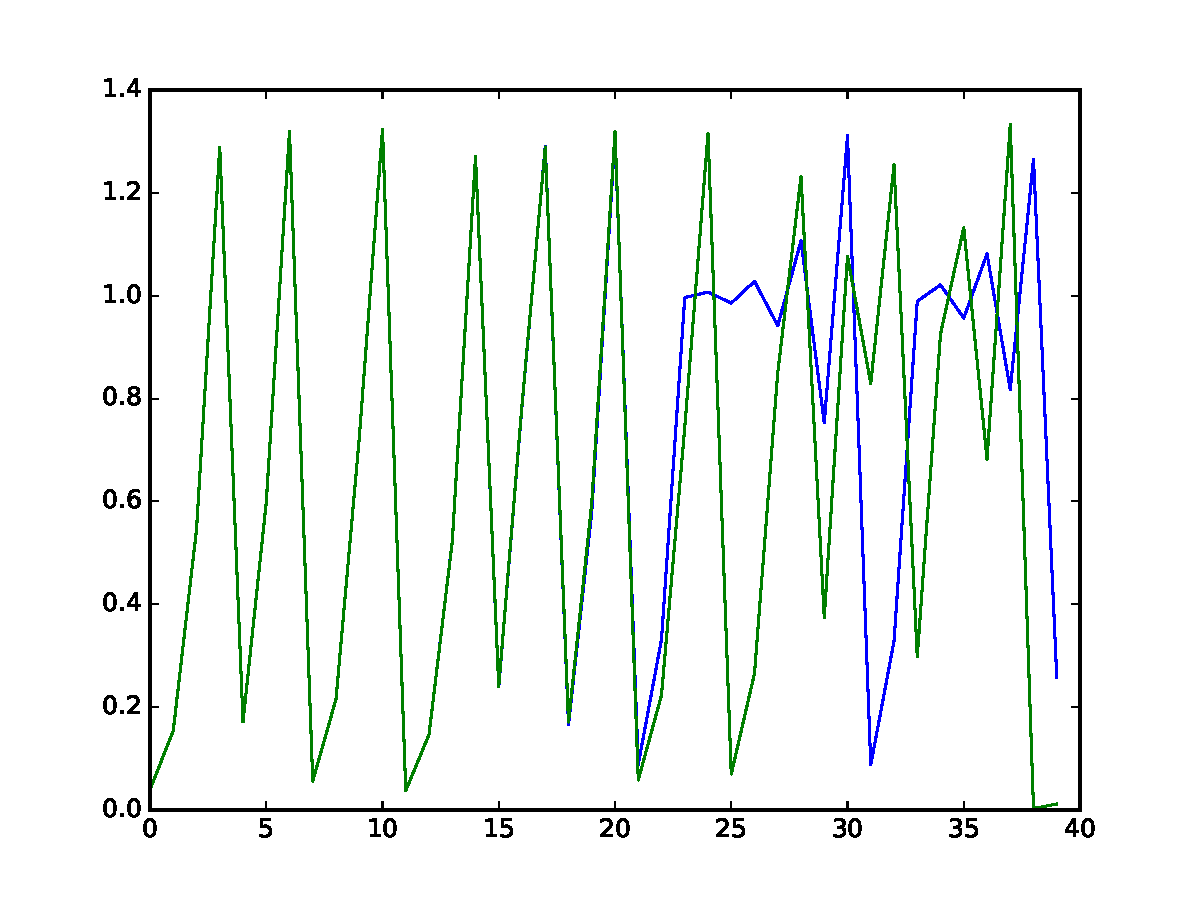
\includegraphics[scale=0.6]{5floats.pdf}
  \caption{Wykres wyników iteracji dla \texttt{Float32} (niebieski) i \texttt{Float64} (zielony)}
\end{figure}

Wyniki drugiej części zadania zostały przedstawione na powyższym wykresie. Dobrze widoczny jest moment, w którym iteracje dla arytmetyki \texttt{Float32} i \texttt{Float64} zaczynają dawać różne rezultaty. Dzieje się tak w okolicach 21. iteracji, kiedy dokładność arytmetyki potrzebna na zapisanie wyników wyrażenia rekurencyjnego staje się niewystarczająca, przez co propagacja błędów daje dla tych dwóch iteracji zupełnie nieskorelowane wyniki. Niższa precyzja arymetyki \texttt{single} spowodowała znacznie szybszą akumulację błędu.
\subsection{Wnioski}
\paragraph{}
Proces sprzężenia zwrotnego jest niestabilny, czyli niewielkie błędy popełnione w początkowym stadium procesu kumulują się w jego kolejnych stadiach. Taka propagacja błędu dla modelu wzrostu populacji jest spowodowana charakterystyką arytmetyk zmiennopozycjnych \texttt{single} i \texttt{double}, na których pracowaliśmy. Błąd wprowadzony na wyjściu stadium procesu będzie dalej kumulowany, przez co kolejne wyniki będą coraz bardziej niewiarygodne. Sposobem chwilowego opóźnienia zbyt dużej akumulacji błędu jest podwyższenie precyzji arytmetyki, jednak nie jest to rozwiązanie wystarczające, gdyż propagowany błąd spowoduje występowanie niepoprawnych wyników w dalszych stadiach procesu.
\section{Zadanie szóste}

\subsection{Opis problemu}
\paragraph{}
Celem zadania było przeprowadzenie eksperymentów dla następującego równania rekurencyjnego:
\begin{center}
$x_{n + 1} = x_{n}^2 + c$ dla $n = 0, 1, ...$
\end{center}

oraz dla zadanych serii danych wejściowych. Eksperymenty polegały na wykonaniu 40 iteracji powyższego wyrażenia i zaobserwowania zachowania generowanych ciągów w arytmetyce \texttt{Float64}.

\subsection{Rozwiązanie}
\paragraph{}
Do przeprowadzenia eksperymentów zostało użyte wyrażenie podane w opisie problemu. Kolejne wartości wyrażenia były generowane iteracyjnie, a kolejne wyniki zostały zapisane w tablicy w celu ich późniejszego odtworzenia.

\subsection{Wyniki i interpretacja}
\paragraph{}
Dla zadanych danych wejściowych eksperymentów można zaobserwować dwa zjawiska: niestabilności związanej ze sprzężeniem zwrotnym oraz stabilizacji układu sprzężenia zwrotnego.

Zacznijmy od omówienia zjawiska stabilizacji układu sprzężenia zwrotnego. Sytuację tę można zaobserwować dla eksperymentów: 1, 2, 4, 5, 6 i 7, jednak z niewielkimi różnicami.

Przykładowo dla eksperymentu: 2. $c = -2$ i $x_{0} = 2$ stabilizacja układu sprzężenia zwrotnego jest już widoczna od samego początku iteracji.

\begin{figure}[htbp]
  \centering
  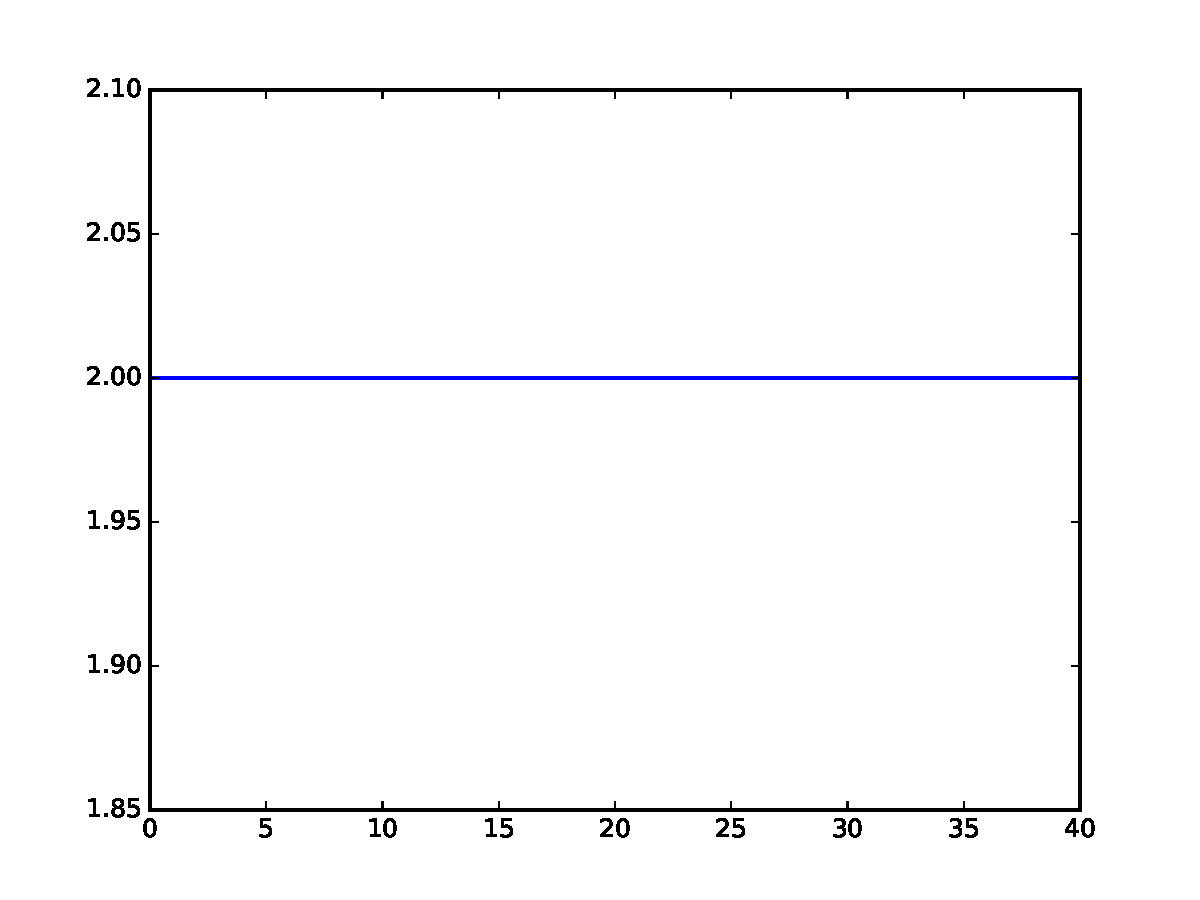
\includegraphics[scale=0.5]{6b.pdf}
  \caption{40 iteracji $x_{n + 1} = x_{n}^2 + c$ dla $n = 0, 1, ...$ dla $c = -2$ i $x_{0} = 2$}
\end{figure}

Natomiast dla eksperymentów 6. $c = -1$ i $x_{0} = 0.75$ i 7. $c = -1$ i $x_{0} = 0.25$ układ sprzężenia zwrotnego wchodzi w stan idealnie stabilny dopiero od pewnej iteracji.

\begin{figure}[htbp]
  \centering
  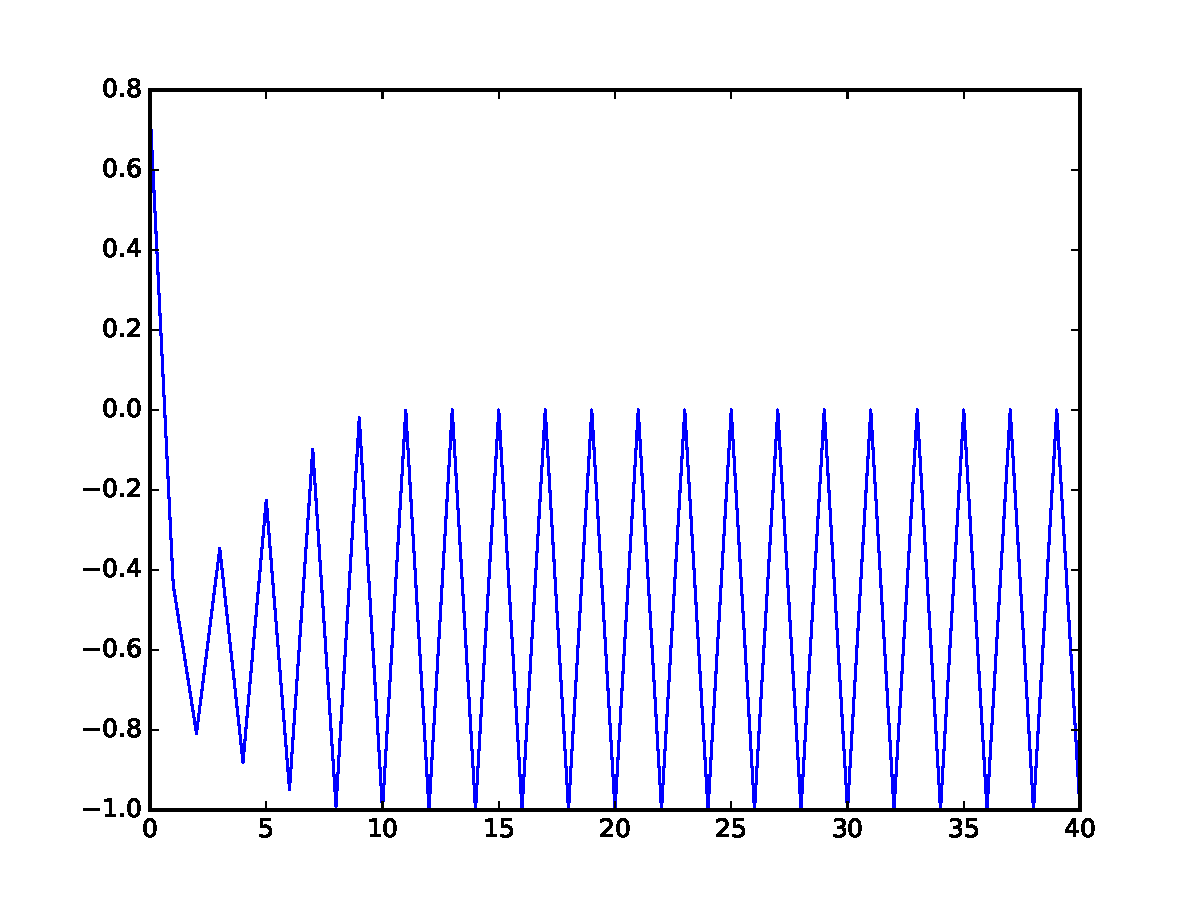
\includegraphics[scale=0.5]{6f.pdf}
  \caption{40 iteracji $x_{n + 1} = x_{n}^2 + c$ dla $n = 0, 1, ...$ dla $c = -1$ i $x_{0} = 0.75$}
\end{figure}
\clearpage
\begin{figure}[htbp]
  \centering
  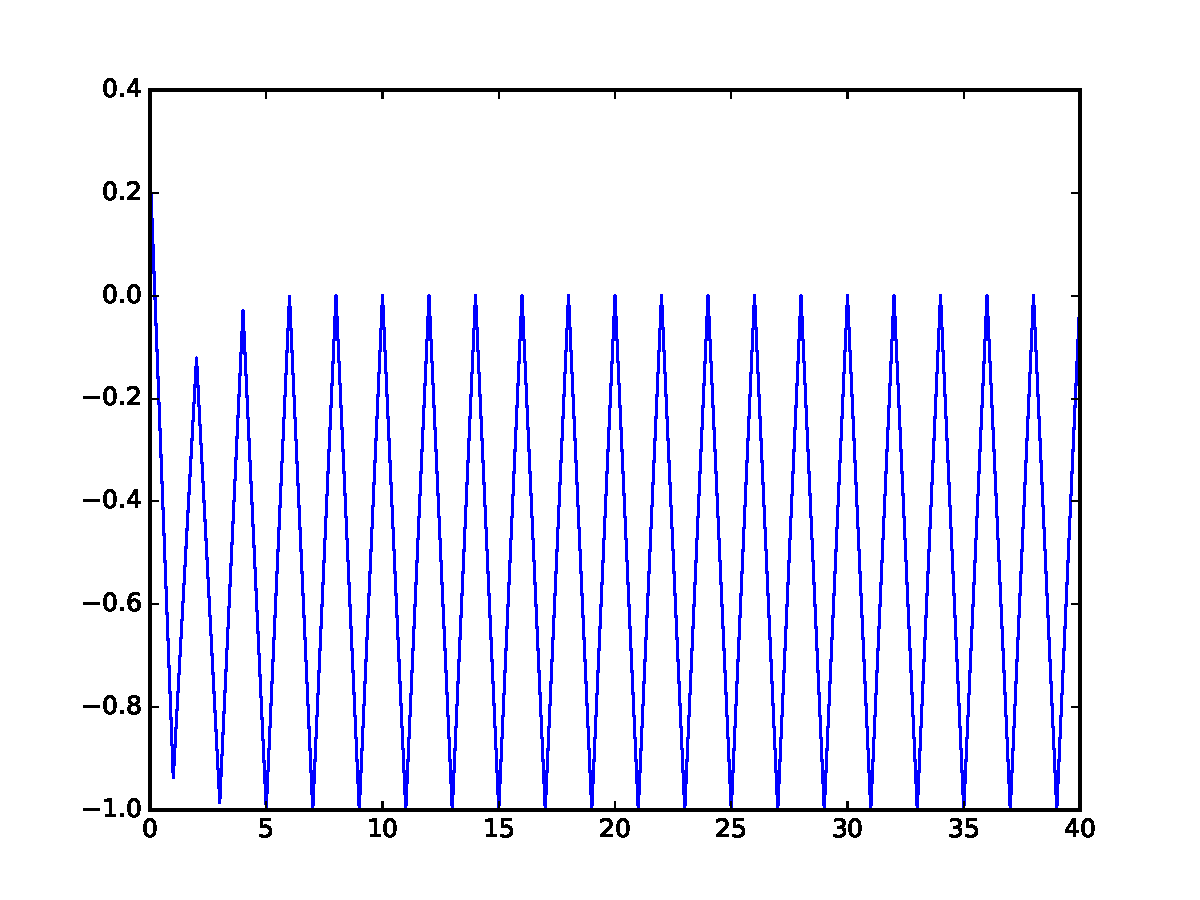
\includegraphics[scale=0.5]{6g.pdf}
  \caption{40 iteracji $x_{n + 1} = x_{n}^2 + c$ dla $n = 0, 1, ...$ dla $c = -1$ i $x_{0} = 0.25$}
\end{figure}

Na widocznych powyżej wykresach stabilizacja układu sprzężenia zwrotnego charakteryzuje się występowaniem przewidywalnych wartości w regularnych interwałach. Jest to swoiste uporządkowanie chaosu.

Dla zadanych eksperymentów pojawia się również niestabilność, podobnie jak w zadaniu 5. Dla eksperymentu 3. $c = -2$ i $x_{0} = 1.99999999999999$ błędy wprowadzone w danych wyjściowych są przekazywane wraz z nimi jako dane wejściowe, co powoduje ich akumulację. Jest to doskonale widoczne na poniższym wykresie.

\begin{figure}[htbp]
  \centering
  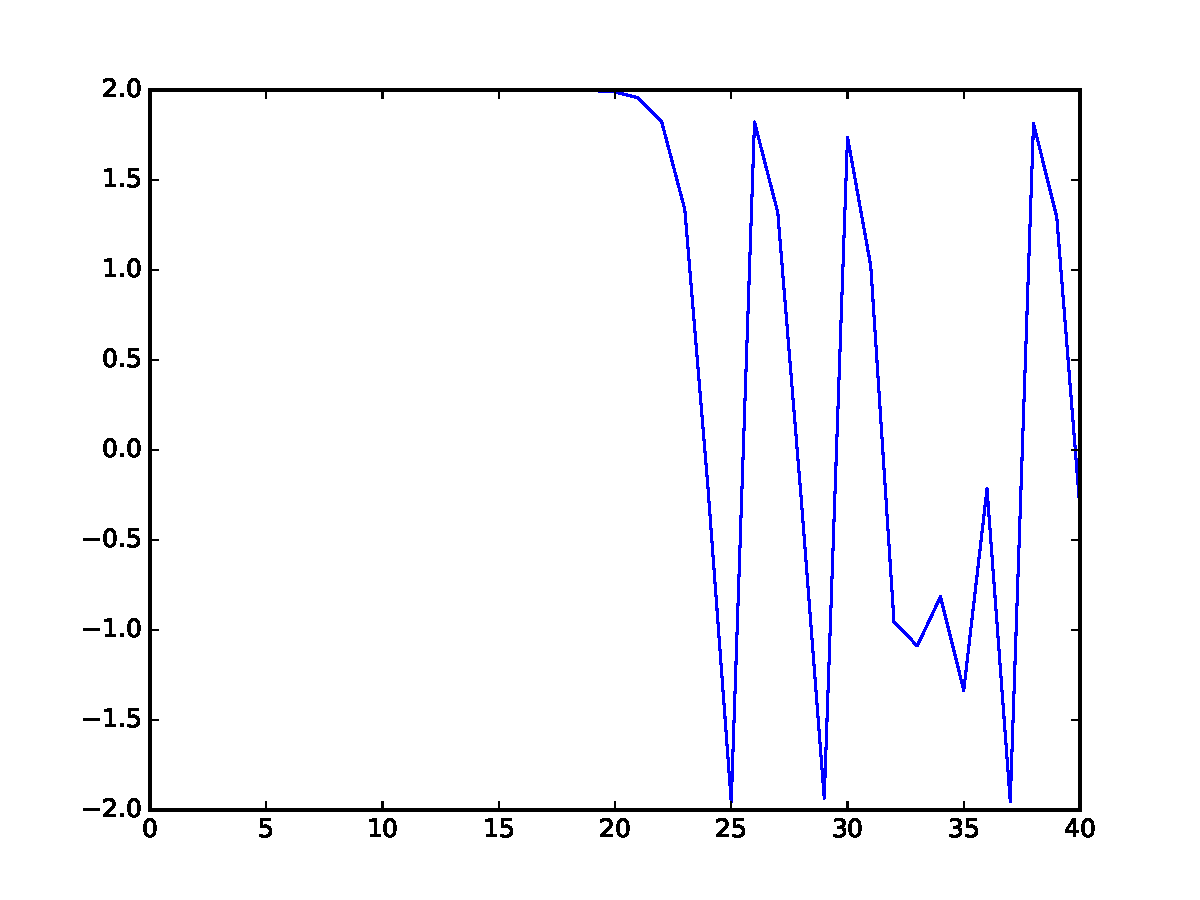
\includegraphics[scale=0.5]{6c.pdf}
  \caption{40 iteracji $x_{n + 1} = x_{n}^2 + c$ dla $n = 0, 1, ...$ dla $c = -2$ i $x_{0} = 1.99999999999999$}
\end{figure}

Od pewnej iteracji wartośc przestają być uporządkowane i stają się nieprzewidywalne. Jest to spodowane akumulacją błędu, wprowadzonego już w początkowych iteracjach.
\subsection{Wnioski}
\paragraph{}
Problem ten pozwolił na zaobserwowanie dwóch zachowań układów sprzężenia zwrotnego: stabilizacji oraz niestabilności. Stabilizację można było zaobserwować jako powtarzanie się przewidywalnych wyników, zaś niestabilność jako generowanie błędnych wyników, spowodowane niewielkimi błędami popełnionymi w początkowych stadiach obliczania wartości wyrażenia. Podobnie jak w zadaniu 5 wprowadzona niestabilność jest skutkiem precyzji arytmetyki \texttt{double}, która była używana do przeprowadzanych w zadaniu obliczeń. Liczba miejsc po przecinku, potrzebnych do przedstawienia kolejnych wyników, zwiększała się, co uniemożliwiało otrzymanie poprawnych wyników.

\end{document}